\documentclass[a4paper,fontset=none]{ctexart}

\usepackage{indentfirst}
\setlength{\parindent}{0em}
\usepackage{autobreak}
\allowdisplaybreaks
\usepackage{parskip}
\usepackage{geometry}
\geometry{top=3cm,bottom=3cm,left=2cm,right=2cm}
\usepackage{anyfontsize}

\usepackage{amsmath}
\usepackage{fontspec}
\usepackage{newpxtext}
\usepackage[slantedGreek,vvarbb]{newpxmath}
\defaultfontfeatures{}
\renewcommand\epsilon\varepsilon
\renewcommand\hbar\hslash
\usepackage{bm}
\renewcommand\mathbf\bm

\setCJKmainfont{SimSun}[BoldFont=Noto Sans CJK SC Medium,ItalicFont=KaiTi]
\setCJKmonofont{Noto Sans Mono CJK SC}[BoldFont=Noto Sans Mono CJK SC Bold,ItalicFont=FangSong]

\usepackage{physics}
\renewcommand\div\divisionsymbol
\usepackage{tikz}
\usetikzlibrary{arrows.meta}
\usetikzlibrary{datavisualization.formats.functions}

\title{\textbf{量子力学作业}}
\author{1900011604\ \ 张植竣\ \ 北京大学}
\date{2022年9月10日}

\begin{document}

\maketitle

    \section*{第一章}

    \begin{itemize}
        \item[5.(a)]
        由波函数的统计诠释得：
        \[
            \int_{-\infty}^{+\infty} \abs{\Psi(x,t)^2} \dd{x} = 1
        \]
        另一方面：
        \begin{align*}
            \int_{-\infty}^{+\infty} \abs{\Psi(x,t)^2} \dd{x}
            &= \int_{-\infty}^{+\infty} A^2 \mathrm{e}^{-2\lambda|x|} \dd{x} \\
            &= 2 \int_{0}^{+\infty} A^2 \mathrm{e}^{-2\lambda x} \dd{x} \\
            &= \frac{A}{\lambda} \int_{0}^{+\infty} \mathrm{e}^{-2\lambda x} \dd(-2\lambda x) \\
            &= \frac{A}{\lambda} \left(\eval{-\mathrm{e}^{-2\lambda x}}_{0}^{+\infty}\right) \\
            &= \frac{A}{\lambda}
        \end{align*}
        则$\dfrac{A}{\lambda} = 1$，$A = \sqrt{\lambda}$。

        \item[5.(b)]
        $x$的平均值为：
        \[
            \expval{x}
            = \int_{-\infty}^{+\infty} x \abs{\Psi(x,t)^2} \dd{x}
            = \int_{-\infty}^{+\infty} \lambda x \mathrm{e}^{-2\lambda|x|} \dd{x}
        \]
        由于$f(x) = \lambda x \mathrm{e}^{-2\lambda|x|}$为奇函数，从$-\infty$到$+\infty$的积分显然为0，则$\expval{x} = 0$。

        $x^2$的平均值为：
        \begin{align*}
            \expval{x^2}
            &= \int_{-\infty}^{+\infty} x^2 \abs{\Psi(x,t)^2} \dd{x} \\
            &= \int_{-\infty}^{+\infty} x^2 \lambda \mathrm{e}^{-2\lambda|x|} \dd{x} \\
            &= 2 \int_{0}^{+\infty} x^2 \lambda \mathrm{e}^{-2\lambda x} \dd{x} \\
            &= \frac{1}{4\lambda^2} \int_{0}^{+\infty} (2\lambda x)^2 \mathrm{e}^{-2\lambda x} \dd(2\lambda x)
        \end{align*}
        令$a=2\lambda x$，使用分部积分法得：
        \begin{align*}
            \int a^2 \mathrm{e}^{-a} \dd{a}
            &= -\int a^2 \dd(\mathrm{e}^{-a}) \\
            &= -a^2 \mathrm{e}^{-a} + \int \mathrm{e}^{-a} \dd(a^2) \\
            &= -a^2 \mathrm{e}^{-a} + 2 \int a \mathrm{e}^{-a} \dd{a} \\
            &= -a^2 \mathrm{e}^{-a} - 2 \int a \dd(\mathrm{e}^{-a}) \\
            &= -a^2 \mathrm{e}^{-a} - 2 \left(a\mathrm{e}^{-a} - \int \mathrm{e}^{-a} \dd{a}\right) \\
            &= -a^2 \mathrm{e}^{-a} - 2 \left(a\mathrm{e}^{-a} + \mathrm{e}^{-a}\right) \\
            &= -\left(a^2 + 2a + 2\right) \mathrm{e}^{-a}
        \end{align*}
        代入$\expval{x^2}$的表达式得：
        \begin{align*}
            \expval{x^2}
            &= \frac{1}{4\lambda^2} \int_{0}^{+\infty} (2\lambda x)^2 \mathrm{e}^{-2\lambda x} \dd(2\lambda x) \\
            &= \frac{1}{4\lambda^2} \left[\eval{-\left(a^2 + 2a + 2\right) \mathrm{e}^{-a}}_0^{+\infty}\right] \\
            &= \frac{1}{2\lambda^2}
        \end{align*}

        \item[5.(c)]
        $x$的标准差为：
        \[
            \sigma = \sqrt{\expval{x^2} - \expval{x}^2} = \frac{\sqrt{2}}{2\lambda}
        \]
        $\abs{\Psi(x,t)^2}$绘图如下：
        \begin{center}
            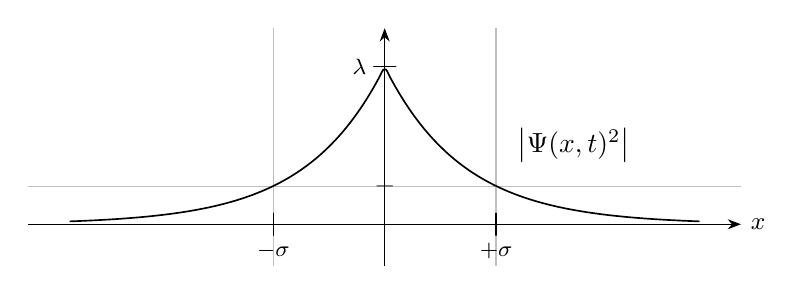
\begin{tikzpicture}[>=Stealth,scale=2]
                \datavisualization [school book axes,
                visualize as smooth line,
                all axes = {ticks=none},
                x axis={ticks and grid={major also at={-0.7071068 as $-\sigma$, 0.7071068 as $+\sigma$}}, label={$x$}},
                y axis={ticks and grid={minor also at={0.2431167}}, ticks={major also at={1 as $\lambda$}}}
                ]
                data [format=function] {
                var x : interval [-2:2] samples 200;
                func y = e^(-2*abs(\value x));
                };
                \draw [node font=small] (1.2,0.5) node {$\abs{\Psi(x,t)^2}$};
            \end{tikzpicture}
        \end{center}
        在$(\expval{x}-\sigma, \expval{x}+\sigma)$范围外发现该粒子的概率为：
        \begin{align*}
            P
            &= \int_{-\infty}^{\expval{x}-\sigma} \abs{\Psi(x,t)^2} \dd{x} + \int_{\expval{x}+\sigma}^{+\infty} \abs{\Psi(x,t)^2} \dd{x} \\
            &= 2 \int_{\tfrac{\sqrt{2}}{2\lambda}}^{+\infty} \lambda \mathrm{e}^{-2\lambda x} \dd{x} \\
            &= \int_{\sqrt{2}}^{+\infty} \mathrm{e}^{-2\lambda x} \dd(2\lambda x) \\
            &= \eval{-\mathrm{e}^{-2\lambda x}}_{\sqrt{2}}^{+\infty} \\
            &= \mathrm{e}^{-\sqrt{2}} \approx 24.31\%
        \end{align*}

        \bigskip
        \item[14.(a)]
        由波函数的统计诠释得：
        \[
            P_{ab}(t) = \int_a^b \abs{\Psi(x,t)^2} \dd{x}
        \]
        上式对时间求导得：
        \begin{align*}
            \dv{P_{ab}}{t}
            &= \int_a^b \pdv{t} \abs{\Psi(x,t)^2} \dd{x} \\
            &= \int_a^b \pdv{t} (\Psi^* \Psi) \dd{x} \\
            &= \int_a^b \pdv{t} \left(\Psi^* \pdv{\Psi}{t} + \Psi \pdv{\Psi^*}{t}\right) \dd{x}
        \end{align*}
        又由Schrödinger方程得：
        \[
            \pdv{\Psi}{t} = \frac{i\hbar}{2m} \pdv[2]{\Psi}{x} - \frac{i}{\hbar}V\Psi
        \]
        同理：
        \[
            \pdv{\Psi^*}{t} = -\frac{i\hbar}{2m} \pdv[2]{\Psi^*}{x} - \frac{i}{\hbar}V\Psi^*
        \]
        则有：
        \[
            \pdv{t}\abs{\Psi(x,t)^2}
            = \frac{i\hbar}{2m} \left(\Psi^* \pdv[2]{\Psi}{x} - \Psi \pdv[2]{\Psi^*}{x}\right)
            = \pdv{x} \left[\frac{i\hbar}{2m} \left(\Psi^* \pdv{\Psi}{x} - \Psi \pdv{\Psi^*}{x}\right)\right]
        \]
        于是$\displaystyle \dv{P_{ab}}{t}$可化为：
        \begin{align*}
            \dv{P_{ab}}{t}
            &= \int_a^b \pdv{t} \Psi^*(x,t) \Psi(x,t) \dd{x} \\
            &= \int_a^b \pdv{x} \left[\frac{i\hbar}{2m} \left(\Psi^* \pdv{\Psi}{x} - \Psi \pdv{\Psi^*}{x}\right)\right] \dd{x} \\
            &= \eval{\frac{i\hbar}{2m} \left(\Psi^* \pdv{\Psi}{x} - \Psi \pdv{\Psi^*}{x}\right)}_a^b \\
            &= J(a,t) - J(b,t)
        \end{align*}
        其中：
        \[
            J(x,t) \equiv \frac{i\hbar}{2m} \left(\Psi \pdv{\Psi^*}{x} - \Psi^* \pdv{\Psi}{x}\right)
        \]
        因为概率是无量纲量，$J(x,t)$的量纲为$\mathrm{T}^{-1}$，则其单位为$\mathrm{s}^{-1}$。

        \item[14.(b)]
        对于波函数$\Psi(x,t) = A \mathrm{e}^{-a(mx^2/\hbar + it)}$，其概率流为：
        \begin{align*}
            J(x,t)
            &= \frac{i\hbar}{2m} \left(\Psi \pdv{\Psi^*}{x} - \Psi^* \pdv{\Psi}{x}\right) \\
            &= \frac{i\hbar}{2m} \left[A \mathrm{e}^{-a(mx^2/\hbar + it)} \cdot \left(-\frac{2amx}{\hbar}\right) A \mathrm{e}^{-a(mx^2/\hbar - it)} - A \mathrm{e}^{-a(mx^2/\hbar - it)} \cdot \left(-\frac{2amx}{\hbar}\right) A \mathrm{e}^{-a(mx^2/\hbar + it)}\right] \\
            &= \frac{i\hbar}{2m} \left[\left(-\frac{2amx}{\hbar}\right) A^2 \mathrm{e}^{-2a(mx^2/\hbar)} - \left(-\frac{2amx}{\hbar}\right) A^2 \mathrm{e}^{-2a(mx^2/\hbar)}\right] \\
            &= 0
        \end{align*}

        \bigskip
        \item[17.(a)]
        由波函数的统计诠释得：
        \[
            P_{ab}(t) = \int_a^b \abs{\Psi(x,t)^2} \dd{x}
        \]
        上式对时间求导得：
        \begin{align*}
            \dv{P_{ab}}{t}
            &= \int_a^b \pdv{t} \abs{\Psi(x,t)^2} \dd{x} \\
            &= \int_a^b \pdv{t} (\Psi^* \Psi) \dd{x} \\
            &= \int_a^b \pdv{t} \left(\Psi^* \pdv{\Psi}{t} + \Psi \pdv{\Psi^*}{t}\right) \dd{x}
        \end{align*}
        又由Schrödinger方程得：
        \[
            \pdv{\Psi}{t} = \frac{i\hbar}{2m} \pdv[2]{\Psi}{x} - \frac{i}{\hbar}(V_0 - i\Gamma)\Psi
        \]
        同理：
        \[
            \pdv{\Psi^*}{t} = -\frac{i\hbar}{2m} \pdv[2]{\Psi^*}{x} - \frac{i}{\hbar}(V_0 + i\Gamma)\Psi^*
        \]
        则有：
        \[
            \pdv{t}\abs{\Psi(x,t)^2}
            = \frac{i\hbar}{2m} \left(\Psi^* \pdv[2]{\Psi}{x} - \Psi \pdv[2]{\Psi^*}{x}\right) - \frac{2\Gamma}{\hbar}\abs{\Psi(x,t)^2}
            = \pdv{x} \left[\frac{i\hbar}{2m} \left(\Psi^* \pdv{\Psi}{x} - \Psi \pdv{\Psi^*}{x}\right)\right] - \frac{2\Gamma}{\hbar}\abs{\Psi(x,t)^2}
        \]
        于是$\displaystyle \dv{P}{t}$可化为：
        \begin{align*}
            \dv{P}{t}
            &= \int_{-\infty}^{+\infty} \pdv{t} \Psi^*(x,t) \Psi(x,t) \dd{x} \\
            &= \int_{-\infty}^{+\infty} \pdv{x} \left[\frac{i\hbar}{2m} \left(\Psi^* \pdv{\Psi}{x} - \Psi \pdv{\Psi^*}{x}\right)\right] \dd{x} - \int_{-\infty}^{+\infty} \frac{2\Gamma}{\hbar}\abs{\Psi(x,t)^2} \dd{x}\\
            &= \eval{\frac{i\hbar}{2m} \left(\Psi^* \pdv{\Psi}{x} - \Psi \pdv{\Psi^*}{x}\right)}_{-\infty}^{+\infty} - \frac{2\Gamma}{\hbar} \int_{-\infty}^{+\infty} \abs{\Psi(x,t)^2} \dd{x} \\
            &= -\frac{2\Gamma}{\hbar} P
        \end{align*}
        这里使用了波函数的性质$\lim\limits_{x \to \infty} \Psi(x,t) = 0$，所以第一个积分的结果：
        \[
            \eval{\frac{i\hbar}{2m} \left(\Psi^* \pdv{\Psi}{x} - \Psi \pdv{\Psi^*}{x}\right)}_{-\infty}^{+\infty}
            = \eval{\frac{i\hbar}{2m} \left(0 \cdot \pdv{\Psi}{x} - 0 \cdot \pdv{\Psi^*}{x}\right)}_{-\infty}^{+\infty}
            = 0
        \]

        \item[17.(b)]
        由$\displaystyle \dv{P}{t} = -\frac{2\Gamma}{\hbar} P$解得：
        \[
            P = P_0 \mathrm{e}^{-\tfrac{2\Gamma}{\hbar} t}
        \]
        其中$P_0$为$t = 0$时的概率值。

        与$P = P_0 \mathrm{e}^{-\tfrac{t}{\tau}}$对比可知，粒子的寿命为：
        \[
            \tau = \frac{\hbar}{2\Gamma}
        \]

        \bigskip
        \item[18.(a)]
        如果固体内自由电子是量子力学的，则需要满足：
        \[
            d \leq \lambda = \frac{h}{\sqrt{3 m_e k_{\mathrm{B}} T}}
        \]
        这给出：
        \[
            T \leq \frac{h^2}{3 m_e k_{\mathrm{B}} d^2}
        \]
        由于典型固体的晶格间距约为$d = 0.3\,\mathrm{nm}$，临界温度为：
        \[
            T_0 = \frac{h^2}{3 m_e k_{\mathrm{B}} d^2} = 1.293 \times 10^{5}\,\mathrm{K}
        \]
        对于固体内的原子核，临界温度应为：
        \[
            T_0 = \frac{h^2}{3 m_{nuc} k_{\mathrm{B}} d^2}
        \]
        以硅晶体为例，原子质量$m_{nuc} = 28.0855\,\mathrm{u} = 4.6637 \times 10^{26}\,\mathrm{kg}$，键长为$d = 0.235\,\mathrm{nm}$，则：
        \[
            T_0 = \frac{h^2}{3 m_{nuc} k_{\mathrm{B}} d^2} = 4.116\,\mathrm{K}
        \]

        \item[18.(b)]
        如果压强$P$下理想气体中的原子是量子力学的，则需要满足：
        \[
            d = \sqrt[3]{\frac{V}{N}} \leq \lambda = \frac{h}{\sqrt{3 m k_{\mathrm{B}} T}}
        \]
        由理想气体状态方程$pV = Nk_{\mathrm{B}}T$得：
        \[
            \sqrt[3]{\frac{k_{\mathrm{B}}T}{p}} \leq \frac{h}{\sqrt{3 m k_{\mathrm{B}} T}}
        \]
        则临界温度为：
        \[
            T_0 = \frac{1}{k_{\mathrm{B}}} \sqrt[5]{\frac{h^6 p^2}{27 m^3}}
        \]
        对于标准大气压下的氦气，$m = 4.0026\,\mathrm{u} = 6.6465 \times 10^{27}\,\mathrm{kg}$，$p = 101325\,\mathrm{Pa}$，临界温度为：
        \[
            T_0 = \frac{1}{k_{\mathrm{B}}} \sqrt[5]{\frac{h^6 p^2}{27 m^3}} = 2.937\,\mathrm{K}
        \]
        对于外太空中的单原子氢，$m = 1.0079\,\mathrm{u}$，$T = 3\,\mathrm{K}$，其de Broglie波长为：
        \[
            \lambda = \frac{h}{\sqrt{3 m k_{\mathrm{B}} T}} = 1.453\,\mathrm{nm}
        \]
        这远小于原子间的平均间距$d = 1\,\mathrm{cm}$，所以该状态下的氢不是量子力学的。
    \end{itemize}

    \newpage
    \section*{第三章}

    \begin{itemize}
        \item[6.]
        根据算符厄米性的定义，需要检验下式是否成立：
        \[
            \bra{f}\ket{\hat{Q}g} = \bra{\hat{Q}f}\ket{g}
        \]
        等号左边可以化为：
        \begin{align*}
            \bra{f}\ket{\hat{Q}g}
            &= \int_0^{2\pi} f^* \dv[2]{g}{\phi} \dd{\phi} \\
            &= \int_0^{2\pi} f^* \dv{\phi}(\dv{g}{\phi}) \dd{\phi} \\
            &= \int_0^{2\pi} f^* \dd(\dv{g}{\phi}) \\
            &= \eval{f^* \dv{g}{\phi}}_0^{2\pi} - \int_0^{2\pi} \dv{g}{\phi} \dd(f^*) \\
            &= -\int_0^{2\pi} \dv{g}{\phi} \dv{f^*}{\phi} \dd{\phi}
        \end{align*}
        注意这里使用了函数的周期性$f(\phi + 2\pi) = f(\phi)$。

        等号右边，使用以下规则：
        \[
            \dv[n]{f^*}{x} = \dv[n]{x}(\Re f - \Im f) = \dv[n]{x}(\Re f) - \dv[n]{x}(\Im f) =\left(\dv[n]{f}{x}\right)^*
        \]
        可以化为：
        \begin{align*}
            \bra{\hat{Q}f}\ket{g}
            &= \int_0^{2\pi} \left(\dv[2]{f}{\phi}\right)^* g \dd{\phi} \\
            &= \int_0^{2\pi} g \dv[2]{f^*}{\phi} \dd{\phi} \\
            &= \int_0^{2\pi} g \dv{\phi}(\dv{f^*}{\phi}) \dd{\phi} \\
            &= \int_0^{2\pi} g \dd(\dv{f^*}{\phi}) \\
            &= \eval{g \dv{f^*}{\phi}}_0^{2\pi} - \int_0^{2\pi} \dv{f^*}{\phi} \dd(g) \\
            &= -\int_0^{2\pi} \dv{f^*}{\phi} \dv{g}{\phi} \dd{\phi}
        \end{align*}
        则$\bra{f}\ket{\hat{Q}g} = \bra{\hat{Q}f}\ket{g}$成立，即$\hat{Q}$是厄米算符。

        为求出该算符的本征方程和本征函数，需要求解以下方程：
        \[
            \hat{Q} f = \dv[2]{f}{\phi} = qf
        \]
        解得本征函数：
        \[
            f = \mathrm{e}^{\pm\sqrt{q}\phi}
        \]
        由函数的周期性边界条件$f(\phi+2\pi) = f(\phi)$得：
        \[
            \mathrm{e}^{\pm\sqrt{q}(\phi+2\pi)}
            = \mathrm{e}^{\pm\sqrt{q}\phi} \cdot \mathrm{e}^{\pm2\pi\sqrt{q}}
            = \mathrm{e}^{\pm\sqrt{q}\phi} \cdot \mathrm{e}^{i(2n\pi)},\quad n \in \mathbb{Z}
        \]
        即：
        \[
            2\pi \sqrt{q} = 2i n \pi,\quad n \in \mathbb{Z}
        \]
        则本征值为：
        \[
            q = -n^2,\quad n = 0,1,2,\cdots
        \]
        算符$\hat{Q}$的谱为：
        \[
            f_n = \mathrm{e}^{\pm in\phi},\quad n = 0,1,2,\cdots
        \]
        每个本征值对应两个本征函数$\mathrm{e}^{\sqrt{q}\phi}$和$\mathrm{e}^{-\sqrt{q}\phi}$（除$n = 0$之外），故$\hat{Q}$的谱是二重简并的。

        \item[16.]
        假设$\{\psi_n(x)\}$是$\hat{P}$和$\hat{Q}$的共同本征函数系，则：
        \[
            \hat{P}\psi_i(x) = p_i \psi_i(x),\quad \hat{Q}\psi_i(x) = q_i \psi_i(x),\quad \forall i \in {1,2,\cdots,n}
        \]
        于是有：
        \begin{align*}
            \comm{\hat{P}}{\hat{Q}} \psi_i(x)
            &= (\hat{P}\hat{Q} - \hat{Q}\hat{P}) \psi_i(x) \\
            &= \hat{P}\hat{Q}\psi_i(x) - \hat{Q}\hat{P}\psi_i(x) \\
            &= pq\psi_i(x) - qp\psi_i(x) \\
            &= 0
        \end{align*}
        如果$\{\psi_n(x)\}$是完备的，即任何Hilbert空间中的函数$f(x)$可以表示成$\psi_i(x)$的线性组合：
        \[
            f(x) = \sum_{i=1}^n c_i \psi_i(x)
        \]
        则有：
        \begin{align*}
            \comm{\hat{P}}{\hat{Q}}f
            &= \comm{\hat{P}}{\hat{Q}}\sum_{i=1}^n c_i \psi_i(x) \\
            &= \sum_{i=1}^n c_i \comm{\hat{P}}{\hat{Q}} \psi_i(x) \\
            &= 0
        \end{align*}
        由于上式对任意的$f(x)$都成立，说明：
        \[
            \comm{\hat{P}}{\hat{Q}} = 0
        \]
    \end{itemize}

\end{document}
